% Created by tikzDevice version 0.12.3.1 on 2021-12-06 10:55:32
% !TEX encoding = UTF-8 Unicode
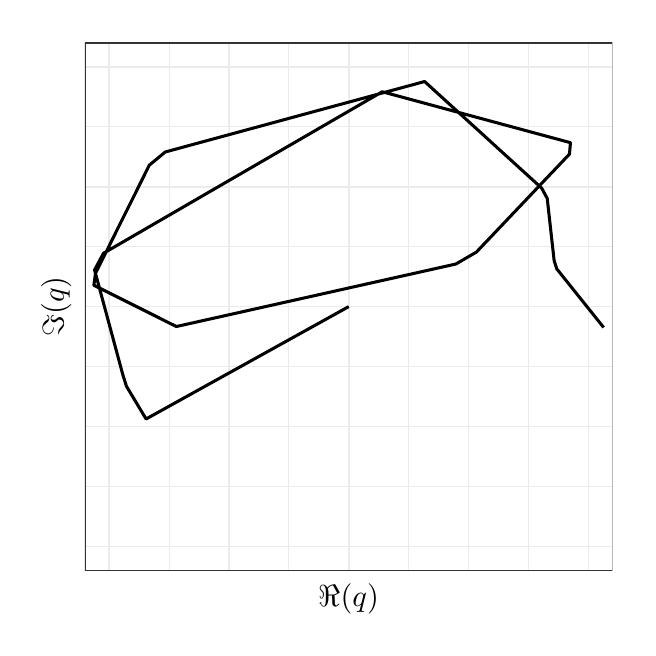
\begin{tikzpicture}[x=1pt,y=1pt]
\definecolor{fillColor}{RGB}{255,255,255}
\path[use as bounding box,fill=fillColor,fill opacity=0.00] (0,0) rectangle (216.81,216.81);
\begin{scope}
\path[clip] (  0.00,  0.00) rectangle (216.81,216.81);
\definecolor{drawColor}{RGB}{255,255,255}
\definecolor{fillColor}{RGB}{255,255,255}

\path[draw=drawColor,line width= 0.6pt,line join=round,line cap=round,fill=fillColor] (  0.00,  0.00) rectangle (216.81,216.81);
\end{scope}
\begin{scope}
\path[clip] ( 20.71, 20.71) rectangle (211.31,211.31);
\definecolor{fillColor}{RGB}{255,255,255}

\path[fill=fillColor] ( 20.71, 20.71) rectangle (211.31,211.31);
\definecolor{drawColor}{gray}{0.92}

\path[draw=drawColor,line width= 0.3pt,line join=round] ( 20.71, 51.04) --
	(211.31, 51.04);

\path[draw=drawColor,line width= 0.3pt,line join=round] ( 20.71, 94.35) --
	(211.31, 94.35);

\path[draw=drawColor,line width= 0.3pt,line join=round] ( 20.71,137.67) --
	(211.31,137.67);

\path[draw=drawColor,line width= 0.3pt,line join=round] ( 20.71,180.99) --
	(211.31,180.99);

\path[draw=drawColor,line width= 0.3pt,line join=round] ( 51.04, 20.71) --
	( 51.04,211.31);

\path[draw=drawColor,line width= 0.3pt,line join=round] ( 94.35, 20.71) --
	( 94.35,211.31);

\path[draw=drawColor,line width= 0.3pt,line join=round] (137.67, 20.71) --
	(137.67,211.31);

\path[draw=drawColor,line width= 0.3pt,line join=round] (180.99, 20.71) --
	(180.99,211.31);

\path[draw=drawColor,line width= 0.6pt,line join=round] ( 20.71, 29.38) --
	(211.31, 29.38);

\path[draw=drawColor,line width= 0.6pt,line join=round] ( 20.71, 72.69) --
	(211.31, 72.69);

\path[draw=drawColor,line width= 0.6pt,line join=round] ( 20.71,116.01) --
	(211.31,116.01);

\path[draw=drawColor,line width= 0.6pt,line join=round] ( 20.71,159.33) --
	(211.31,159.33);

\path[draw=drawColor,line width= 0.6pt,line join=round] ( 20.71,202.65) --
	(211.31,202.65);

\path[draw=drawColor,line width= 0.6pt,line join=round] ( 29.38, 20.71) --
	( 29.38,211.31);

\path[draw=drawColor,line width= 0.6pt,line join=round] ( 72.69, 20.71) --
	( 72.69,211.31);

\path[draw=drawColor,line width= 0.6pt,line join=round] (116.01, 20.71) --
	(116.01,211.31);

\path[draw=drawColor,line width= 0.6pt,line join=round] (159.33, 20.71) --
	(159.33,211.31);

\path[draw=drawColor,line width= 0.6pt,line join=round] (202.65, 20.71) --
	(202.65,211.31);
\definecolor{drawColor}{RGB}{0,0,0}

\path[draw=drawColor,line width= 1.1pt,line join=round] (208.13,108.48) --
	(206.01,111.12) --
	(203.89,113.77) --
	(201.77,116.42) --
	(199.66,119.07) --
	(197.54,121.71) --
	(195.42,124.36) --
	(193.30,127.01) --
	(191.18,129.65) --
	(190.23,132.67) --
	(189.88,135.87) --
	(189.52,139.08) --
	(189.16,142.28) --
	(188.81,145.48) --
	(188.45,148.68) --
	(188.09,151.88) --
	(187.74,155.09) --
	(185.74,158.83) --
	(180.45,163.64) --
	(175.16,168.46) --
	(169.87,173.27) --
	(164.59,178.09) --
	(159.30,182.90) --
	(154.01,187.72) --
	(148.72,192.53) --
	(143.44,197.35) --
	(131.72,194.17) --
	(120.00,190.98) --
	(108.29,187.80) --
	( 96.57,184.62) --
	( 84.85,181.43) --
	( 73.14,178.25) --
	( 61.42,175.07) --
	( 49.70,171.88) --
	( 43.95,167.11) --
	( 41.17,161.53) --
	( 38.39,155.95) --
	( 35.62,150.38) --
	( 32.84,144.80) --
	( 30.07,139.23) --
	( 27.29,133.65) --
	( 24.52,128.08) --
	( 23.91,123.74) --
	( 27.64,121.87) --
	( 31.37,120.01) --
	( 35.10,118.14) --
	( 38.83,116.28) --
	( 42.56,114.41) --
	( 46.28,112.55) --
	( 50.01,110.68) --
	( 53.74,108.82) --
	( 66.37,111.64) --
	( 78.99,114.46) --
	( 91.62,117.29) --
	(104.24,120.11) --
	(116.87,122.94) --
	(129.49,125.76) --
	(142.12,128.58) --
	(154.74,131.41) --
	(162.15,135.72) --
	(166.96,140.77) --
	(171.76,145.83) --
	(176.56,150.89) --
	(181.36,155.94) --
	(186.16,161.00) --
	(190.97,166.06) --
	(195.77,171.11) --
	(196.14,175.25) --
	(187.63,177.55) --
	(179.13,179.85) --
	(170.63,182.15) --
	(162.12,184.45) --
	(153.62,186.75) --
	(145.12,189.05) --
	(136.62,191.35) --
	(128.11,193.65) --
	(115.52,186.36) --
	(102.93,179.06) --
	( 90.34,171.77) --
	( 77.75,164.47) --
	( 65.16,157.18) --
	( 52.57,149.88) --
	( 39.98,142.59) --
	( 27.39,135.29) --
	( 24.17,129.25) --
	( 25.63,123.84) --
	( 27.09,118.43) --
	( 28.55,113.02) --
	( 30.01,107.61) --
	( 31.47,102.20) --
	( 32.93, 96.79) --
	( 34.39, 91.38) --
	( 35.70, 87.21) --
	( 36.72, 85.52) --
	( 37.73, 83.84) --
	( 38.74, 82.15) --
	( 39.75, 80.47) --
	( 40.77, 78.78) --
	( 41.78, 77.10) --
	( 42.79, 75.41) --
	(116.01,116.01);
\definecolor{drawColor}{gray}{0.20}

\path[draw=drawColor,line width= 0.6pt,line join=round,line cap=round] ( 20.71, 20.71) rectangle (211.31,211.31);
\end{scope}
\begin{scope}
\path[clip] (  0.00,  0.00) rectangle (216.81,216.81);
\definecolor{drawColor}{RGB}{0,0,0}

\node[text=drawColor,anchor=base,inner sep=0pt, outer sep=0pt, scale=  1.10] at (116.01,  7.64) {$\Re(q)$};
\end{scope}
\begin{scope}
\path[clip] (  0.00,  0.00) rectangle (216.81,216.81);
\definecolor{drawColor}{RGB}{0,0,0}

\node[text=drawColor,rotate= 90.00,anchor=base,inner sep=0pt, outer sep=0pt, scale=  1.10] at ( 13.08,116.01) {$\Im(q)$};
\end{scope}
\end{tikzpicture}
